\documentclass{beamer}
\usepackage{listings}
\lstset{
%language=C,
frame=single, 
breaklines=true,
columns=fullflexible
}
\usepackage{subcaption}
\usepackage{url}

\usepackage{tikz}
\usetikzlibrary{arrows.meta,positioning}
\usepackage{pgfplots}
\pgfplotsset{compat=1.17}
\usepackage{tkz-fct}
\usepackage{mathrsfs}
\usepackage{txfonts}
\usepackage{tkz-euclide} 
\usetikzlibrary{calc,math}
\usepackage{float}
\newcommand\norm[1]{\left\lVert#1\right\rVert}
\renewcommand{\vec}[1]{\mathbf{#1}}
\providecommand{\pr}[1]{\ensuremath{\Pr\left(#1\right)}}
\usepackage[export]{adjustbox}
\usepackage[utf8]{inputenc}
\usepackage{amsmath}
\usetheme{Boadilla}
\title{AI1103 Project}
\author{Amulya Tallamraju - AI20BTECH11003}
\date{}
\begin{document}
\begin{frame}
\titlepage
\end{frame}
\section{}
\begin{frame}{Design and BER Performance  Analysis of MIMO and Massive MIMO Networks under Perfect and Imperfect CSI }
\begin{block}{Abstract}
With  upcoming  5G networks, higher data rate and higher    capacity    are   required   for   a   commercial wireless communication  system.
After sternly affecting  bit  error  rate  of  communication  system,  multipath fading  in  wireless communication system also gives weak signal strength. 
Multi input- multi output (MIMO) and Massive MIMO  system is used to overcome this drawback. This  research  paper  presents  the  salient features of MIMO  and massive MIMO  networks and  investigates its  BER  performance  under  AWGN  (  white Gaussian noise) and Rayleigh  fading  communication  channel  under  the  effects  of perfect  and  imperfect  channel  state  information  (CS I)  modes, along with the consideration of trials and prospects.
\end{block}
\end{frame}
\section{Introduction}
\begin{frame}{Challenges for wireless communication system.}
\begin{figure}
    \centering
    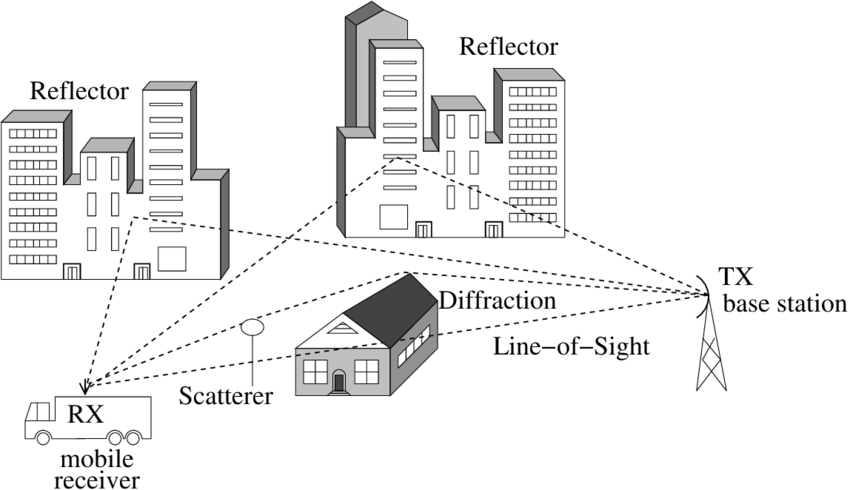
\includegraphics[width=0.5\columnwidth]{Multipath-propagation-of-electromagnetic-waves.png}
    \caption{Multipath propagation}
    \label{fig:my_label}
\end{figure}

\begin{itemize}
\item No guiding medium between transmitter and receiver.\\
\item Multiple signals superpose at the receiver. As a result of destructive interference, strength of signal fades(weakens). This effect is known as fading.
\end{itemize}

\end{frame}
\begin{frame}{MIMO}
\textbf{MIMO - Multiple Input Multiple Output}\\
The MIMO system leads to a significant increase
in the data rates.\\
It is a
combination of Multiple Transmit Antennas at the transmitter and Multiple Receive Antennas at the receiver.\\
A MIMO system is a collection of a large number of fading Channels one between
each transmit antenna and each receive antenna pair. 

\begin{figure}
    \centering
    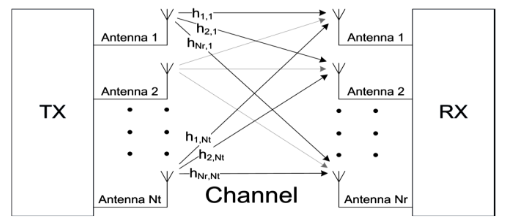
\includegraphics[width=0.6\columnwidth]{MIMO block diagram.PNG}
    \caption{MIMO BLOCK DIAGRAM}
    \label{2}
\end{figure}
\end{frame}
\begin{frame}{Massive MIMO}

Massive MIMO — which is an extension of MIMO — expands beyond the legacy systems by adding a much higher number of antennas on the base station. The “massive” number of antennas helps focus energy, which brings drastic improvements in throughput and efficiency. 

\begin{figure}
    \centering
    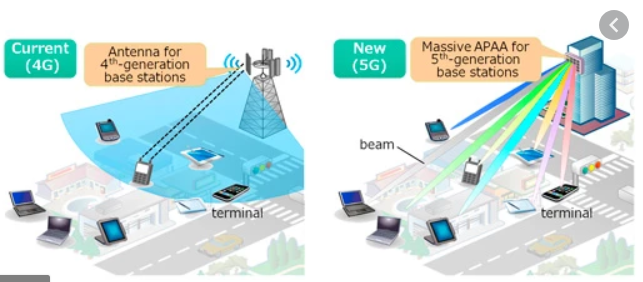
\includegraphics[width=0.8\columnwidth]{mmimo.PNG}
    \caption{4G v/s 5G}
    \label{3}
\end{figure}
\end{frame}
\begin{frame}{Channel state information}
Channel state information (CSI) refers to known channel properties of a communication link. This information describes how a signal propagates from the transmitter to the receiver.\\
There are basically two levels of CSI, namely instantaneous CSI and statistical CSI. 
\begin{block}{}
\begin{itemize}
    \item \textbf{Instantaneous CSI (Perfect)} means that the current channel conditions are known.This can be used to optimize the received signal to achieve low bit error rates.
    \item \textbf{Statistical CSI (Imperfect)} means that a statistical characterization of the channel is known. This description can include, for example, the type of fading distribution.
\end{itemize}
The CSI acquisition is practically limited by how fast the channel conditions are changing. 
\end{block}
\end{frame}
\begin{frame}{Rayleigh Distribution }
\begin{block}{}
 The probability density function of the Rayleigh distribution is
\begin{align}
    { f(x;\sigma )={\frac {x}{\sigma ^{2}}}e^{-x^{2}/(2\sigma ^{2})},\quad x\geq 0,}  
\end{align}
where  $\sigma$ is the scale parameter of the distribution.
\end{block}
  \begin{figure}
    \centering
    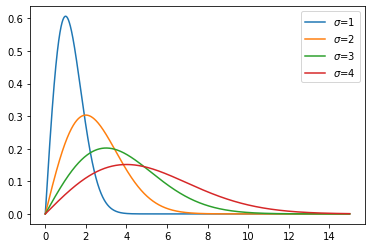
\includegraphics[width=0.5\columnwidth]{Rayleigh DIstribution.png}
    \caption{Pdf of Rayleigh Distribution for different values of $\sigma$}
    \label{4}
\end{figure}   
\end{frame}
\begin{frame}{Rayleigh fading Channel}
The fading channel coefficient h depends on factors like attenuation ($a_i$) and time delay($\tau_i$) associated with the channel. 
\begin{block}{Modelling the distribution of the fading channel coefficient}
\begin{align}
    h&=\sum_{i=0}^{L-1}a_i\exp{(-j2\pi f_c \tau_i)}\\
    &=\sum_{i=0}^{L-1}a_i\cos{(2\pi f_c \tau_i)}-j\sum_{i=0}^{L-1}a_i\sin{(2\pi f_c \tau_i)}\\
    &=X+jY
\end{align}
where X=$\sum_{i=0}^{L-1}a_i\cos{(2\pi f_c \tau_i)}$ and Y=$-\sum_{i=0}^{L-1}a_i\sin{(2\pi f_c \tau_i)}$
\end{block}
\end{frame}
\begin{frame}{}
 As X and Y are the sums of a large number
of independent random variables, by the central limit theorem X and Y can be
assumed to be Gaussian distributed random variables.
\begin{block}{Joint Pdf of X and Y}
\begin{align}
&X,Y\sim \mathcal{N}(\mu ,\sigma^2)\\
f_X(x)=&\frac{1}{\sqrt{2\pi \sigma^2}}exp{\frac{-(x-\mu)^2}{2\sigma^2}}\\
f_Y(y)=&\frac{1}{\sqrt{2\pi \sigma^2}}exp{\frac{-(y-\mu)^2}{2\sigma^2}}
\end{align}
Assuming X and Y are independent random variables and substituting $\mu=0$ for simplification 
\begin{align}
f_{XY}(x,y)=&\frac{1}{{2\pi \sigma^2 }}exp{\left(-(x^2+y^2)\right)}  \label{eq1} 
\end{align}
\end{block}
\end{frame}
\begin{frame}{}

\begin{block}{ Distribution of the fading channel in terms of its Amplitude and phase using Jacobian }
\begin{align}
&h=x+jy=ae^{j\phi}\\
&a=\sqrt{x^2+y^2}, \phi=\tan^{-1}{\frac{y}{x}}\label{eq2}\\
&f_{A,{\Phi}}(a,\phi)=f_{XY}(x,y)\big{|}J_{XY}\big{|}\\
&\big{|}J_{XY}\big{|} =
\begin{vmatrix}
\frac{\partial x}{\partial a} & \frac{\partial y}{\partial a} \\
\frac{\partial x}{\partial \phi} & \frac{\partial y}{\partial \phi} 
\end{vmatrix}=\begin{vmatrix}
\cos{\phi} & \sin{\phi} \\
-a\sin{\phi} & a\cos{\phi} 
\end{vmatrix}\label{eq3}
\end{align}
from \eqref{eq1},\eqref{eq2} and \eqref{eq3} we get
\begin{align}
  &f_{A,{\Phi}}(a,\phi)= \frac{a}{{2\pi \sigma^2}}\exp{\left(\frac{-a^2}{2\sigma^2}\right)} 
\end{align}
\end{block}
\end{frame}
\begin{frame}{}
 \begin{block}{Marginal distribution of A}
 \begin{align}
   f_A(a)&=\int_{-\pi}^{\pi}f_{A,{\Phi}}(a,\phi)\;d\phi\\
   &= \int_{-\pi}^{\pi}\frac{a}{{2\pi \sigma^2}}\exp{\left(\frac{-a^2}{2\sigma^2}\right)}\;d\phi\\
   &=\frac{a}{\sigma^2}\exp{\left(\frac{-a^2}{2\sigma^2}\right)}
 \end{align}
 \end{block}
 Thus the coefficient follows the Rayleigh distribution and is fading in nature. It is therefore called as a Rayleigh fading channel.
\end{frame}
\begin{frame}{AWGN}

Additive white Gaussian noise (AWGN) is a basic noise model used in information theory to mimic the effect of many random processes that occur in nature. The modifiers denote specific characteristics:
\begin{block}{}
\begin{itemize}
    \item Additive because it is added to any noise that might be intrinsic to the information system.
    \item White refers to the idea that the noise has the same power distribution at every frequency.
    \item Gaussian because it has a normal distribution in the time domain with an average time domain value of zero.

\end{itemize}
\end{block}
\begin{figure}
    \centering
    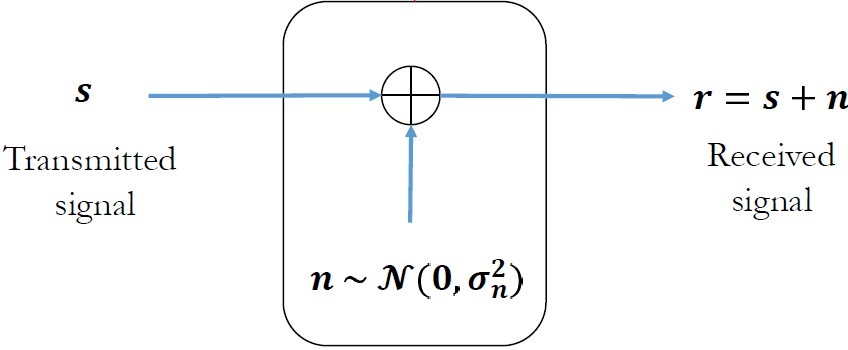
\includegraphics[width=0.4\columnwidth]{awgn.jpg}
    \caption{AWGN Channel}
    \label{5}
\end{figure}
\end{frame}


\begin{frame}{BPSK Modulation }

    \begin{block}{BPSK}
    BPSK stands for binary phase shift keying in which the information symbol 0 is modulated with an amplitude level  $\sqrt{P} $ and the information symbol 1 is modulated with an
amplitude level - $\sqrt{P} $. So, we have 2 voltage levels  $\sqrt{P} $ and -  $\sqrt{P} $ . So, there are 2
phases the phase of  $\sqrt{P} $ is 0 and the phase of -  $\sqrt{P} $ is 180 degrees.
At the receiver:\\
If received symbol $\geq 0 \rightarrow 0$ \\
If received symbol $< 0 \rightarrow 1$
    \end{block}
\end{frame}
\begin{frame}{BER}
Bit error rate (BER) is defined as the percentage of bits that have errors relative to the total number of bits received in a transmission. 
    \begin{block}{AWGN Channel}
    The symbols 0 and 1 are equiprobable hence it suffices to calculate the bit error rate as the probability that the received signal is 1 when the transmitted signal is 0.
    \begin{align}
    y&=x+n\\
        P_e&=\pr{\sqrt{P}+n<0 }\\
        &=\pr{\sqrt{P}<-n }=\pr{\sqrt{P}<n }
    \end{align}
    Since n has a symmetric pdf. Let $w\sim \mathcal{N}(0,1)$.Then $n=\sigma w$
    \begin{align}
     P_e&=\pr{\sqrt{\frac{P}{\sigma^2}}<w }
    \end{align}
    \end{block}
\end{frame}
\begin{frame}{}
\begin{block}{BER of AWGN in terms of Q function}
\begin{align}
     P_e&=\pr{\sqrt{\frac{P}{\sigma^2}}<w }\\
     &=Q\left(\sqrt{\frac{P}{\sigma^2}}\right)\\
     &=Q\left(\sqrt{SNR}\right) \label{6}
    \end{align}
  where \begin{align}
    Q(x)& = \frac{1}{\sqrt{2\pi}} \int_x^\infty \exp\left(-\frac{u^2}{2}\right) \, du.\\
    SNR &=\frac{P_{signal}}{E[N^2]}=\frac{P}{\sigma^2}
  \end{align}
\end{block}
\end{frame}
\begin{frame}{BER Analysis for Rayleigh Fading Channel}
    \begin{block}{}
   For a wireless communication system
   \begin{align}
     y=hx+n  
   \end{align}
   where h is the fading channel coefficient following Rayleigh distribution and n is awgn.\\
   Received signal power = $|h|^2 P$
but $h = ae^{j\phi}$.
 Therefore, we have
Received power = $a^2P$
\begin{align}
    SNR_F =\frac{a^2P}{\sigma^2}= a^2SNR
\end{align}
From \eqref{6}
\begin{align}
   P_e(a)&=Q(\sqrt{SNR_F}) \\
   &=Q(\sqrt{a^2SNR})
\end{align}
    \end{block}
\end{frame}
\begin{frame}{}
\begin{block}{BER expression for rayleigh fading channel}
 But, because of the random nature of the fading channel
coefficient $a^2SNR$ is also a random quantity. Therefore, average bit error rate is given by
 \begin{align}
  P_e&=E[P_e(A)]\\
      &=\int_0^{\infty}Q(\sqrt{a^2SNR})f_A(a) \, da\\
    &=\frac{1}{2}\left(1-\sqrt{\frac{SNR}{2+SNR}}\right)
 \end{align}

  \end{block}
\end{frame}
\begin{frame}{BER Analysis}
 \begin{figure}
\centering
\begin{minipage}{.5\textwidth}
  \centering
  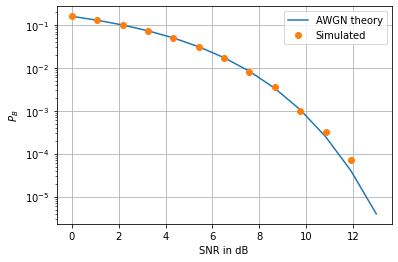
\includegraphics[width=\columnwidth]{ber awgn.png}
  \caption{BER of AWGN under BPSK modulation}
  \label{fig:test3}
\end{minipage}%
\begin{minipage}{.5\textwidth}
  \centering
  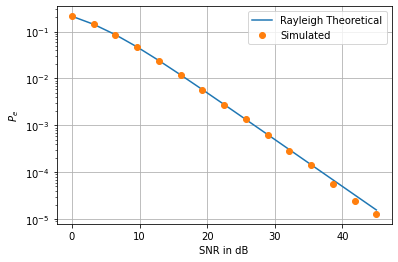
\includegraphics[width=\columnwidth]{ber rayleigh.png}
  \caption{BER of Rayleigh fading channel with AWGN}
  \label{fig:test4}
\end{minipage}
\end{figure}   
\end{frame}
\begin{frame}{ZF and MRC}
    \begin{block}{Zero Forcing}
     This  is  used  for  the retrieval  of  the  original  signal  by choosing $\Bar{x}$ that minimises $\norm{\bar{y}-H\bar{x}}^2$ . The main aim of Zero forcing is to  improve the performance of the system by bringing the inter-symbol interference to zero.
    \end{block}
    \begin{block}{Maximum Ratio Combining}
     This technique is employed to maximise the SNR. The output is taken as the weighted output of various received signals. For maximising the SNR, the weight vector is taken to be proportional to the channel coefficients vector.
    \end{block}
\end{frame}
\begin{frame}{Conclusion}
\begin{figure}
\centering
\begin{minipage}{.5\textwidth}
  \centering
  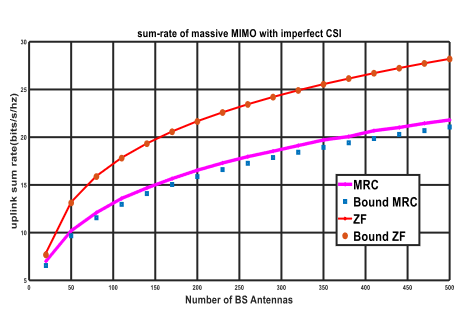
\includegraphics[width=\columnwidth]{sum rates of massive mimo imperfect CSI.PNG}
  \caption{sum rates of massive mimo imperfect CSI}
  \label{fig:test1}
\end{minipage}%
\begin{minipage}{.5\textwidth}
  \centering
  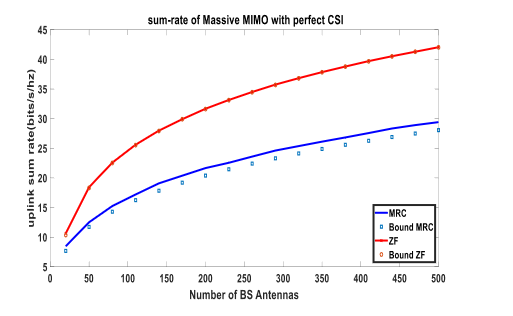
\includegraphics[width=\columnwidth]{sum rates of massive mimo perfect CSI.PNG}
  \caption{sum rates of massive mimo perfect CSI}
  \label{fig:test2}
\end{minipage}
\end{figure}
 MIMO  system performance  has  increased  under  ZF  mode  when  seen  both under perfect and imperfect CSI. 
\end{frame}
\end{document}